The 2010 Affordable Care Act (ACA) required states to expand their Medicaid eligibility requirements by 2014 to offer coverage to all adults with incomes at or below 138 percent of the federal poverty level (FPL). The United States Supreme Court ruled this requirement unconstitutional in 2012, allowing states to decide whether to expand Medicaid coverage. In 2014, twenty-six states and the District of Columbia expanded their Medicaid programs. From 2015 through 2020 an additional twelve states elected to expand their Medicaid programs. This first wave of expansions in 2014 enabled researchers to examine the effects of Medicaid expansion by using expansion states as ``treated'' states and non-expansion states as ``control'' states. Our primary goal in this paper is to estimate the effect of 2014 Medicaid expansion on non-elderly adult uninsurance rates among states that did not expand Medicaid. 

We pay particular attention to one potential source of effect heterogeneity: Republican governance. Medicaid take-up rates are lower than 100 percent and historically have varied across states. This variation is partly a function of state discretion in administering programs: for example, program outreach, citizenship verification policies, and application processes differ across states (\cite{courtemanche2017early}). Here we consider how political composition may have driven differences in take-up rates between states. Prior to the 2014 Medicaid expansion, \cite{sommers2012understanding} found that conservative political ideology was associated with lower Medicaid enrollment rates, even after controlling for a variety of other policies. Most importantly, political ideology appears to have largely driven a state's decision to expand Medicaid in 2014. Figure~\ref{fig:stateideology} plots a measure of each state's 2013 institutional ideology score (\cite{berry1998measuring}) by their Medicaid expansion status. Higher values of this score correspond to more liberal government institutions. The red dashed line indicates the mean expansion state score and the gray dashed line indicates the mean non-expansion state score. Figure~\ref{fig:stateideology} illustrates that non-expansion states are more conservative than expansion states. If the differential take-up rates observed by \cite{sommers2012understanding} continue to hold post-expansion, we should expect this differential to reduce the absolute magnitude of the estimated treatment effect on non-expansion states relative to expansion states (conditional on any other variables).

\begin{figure}[H]
    \begin{center}
    \caption{Government ideology and Medicaid expansion}
    \label{fig:stateideology}
    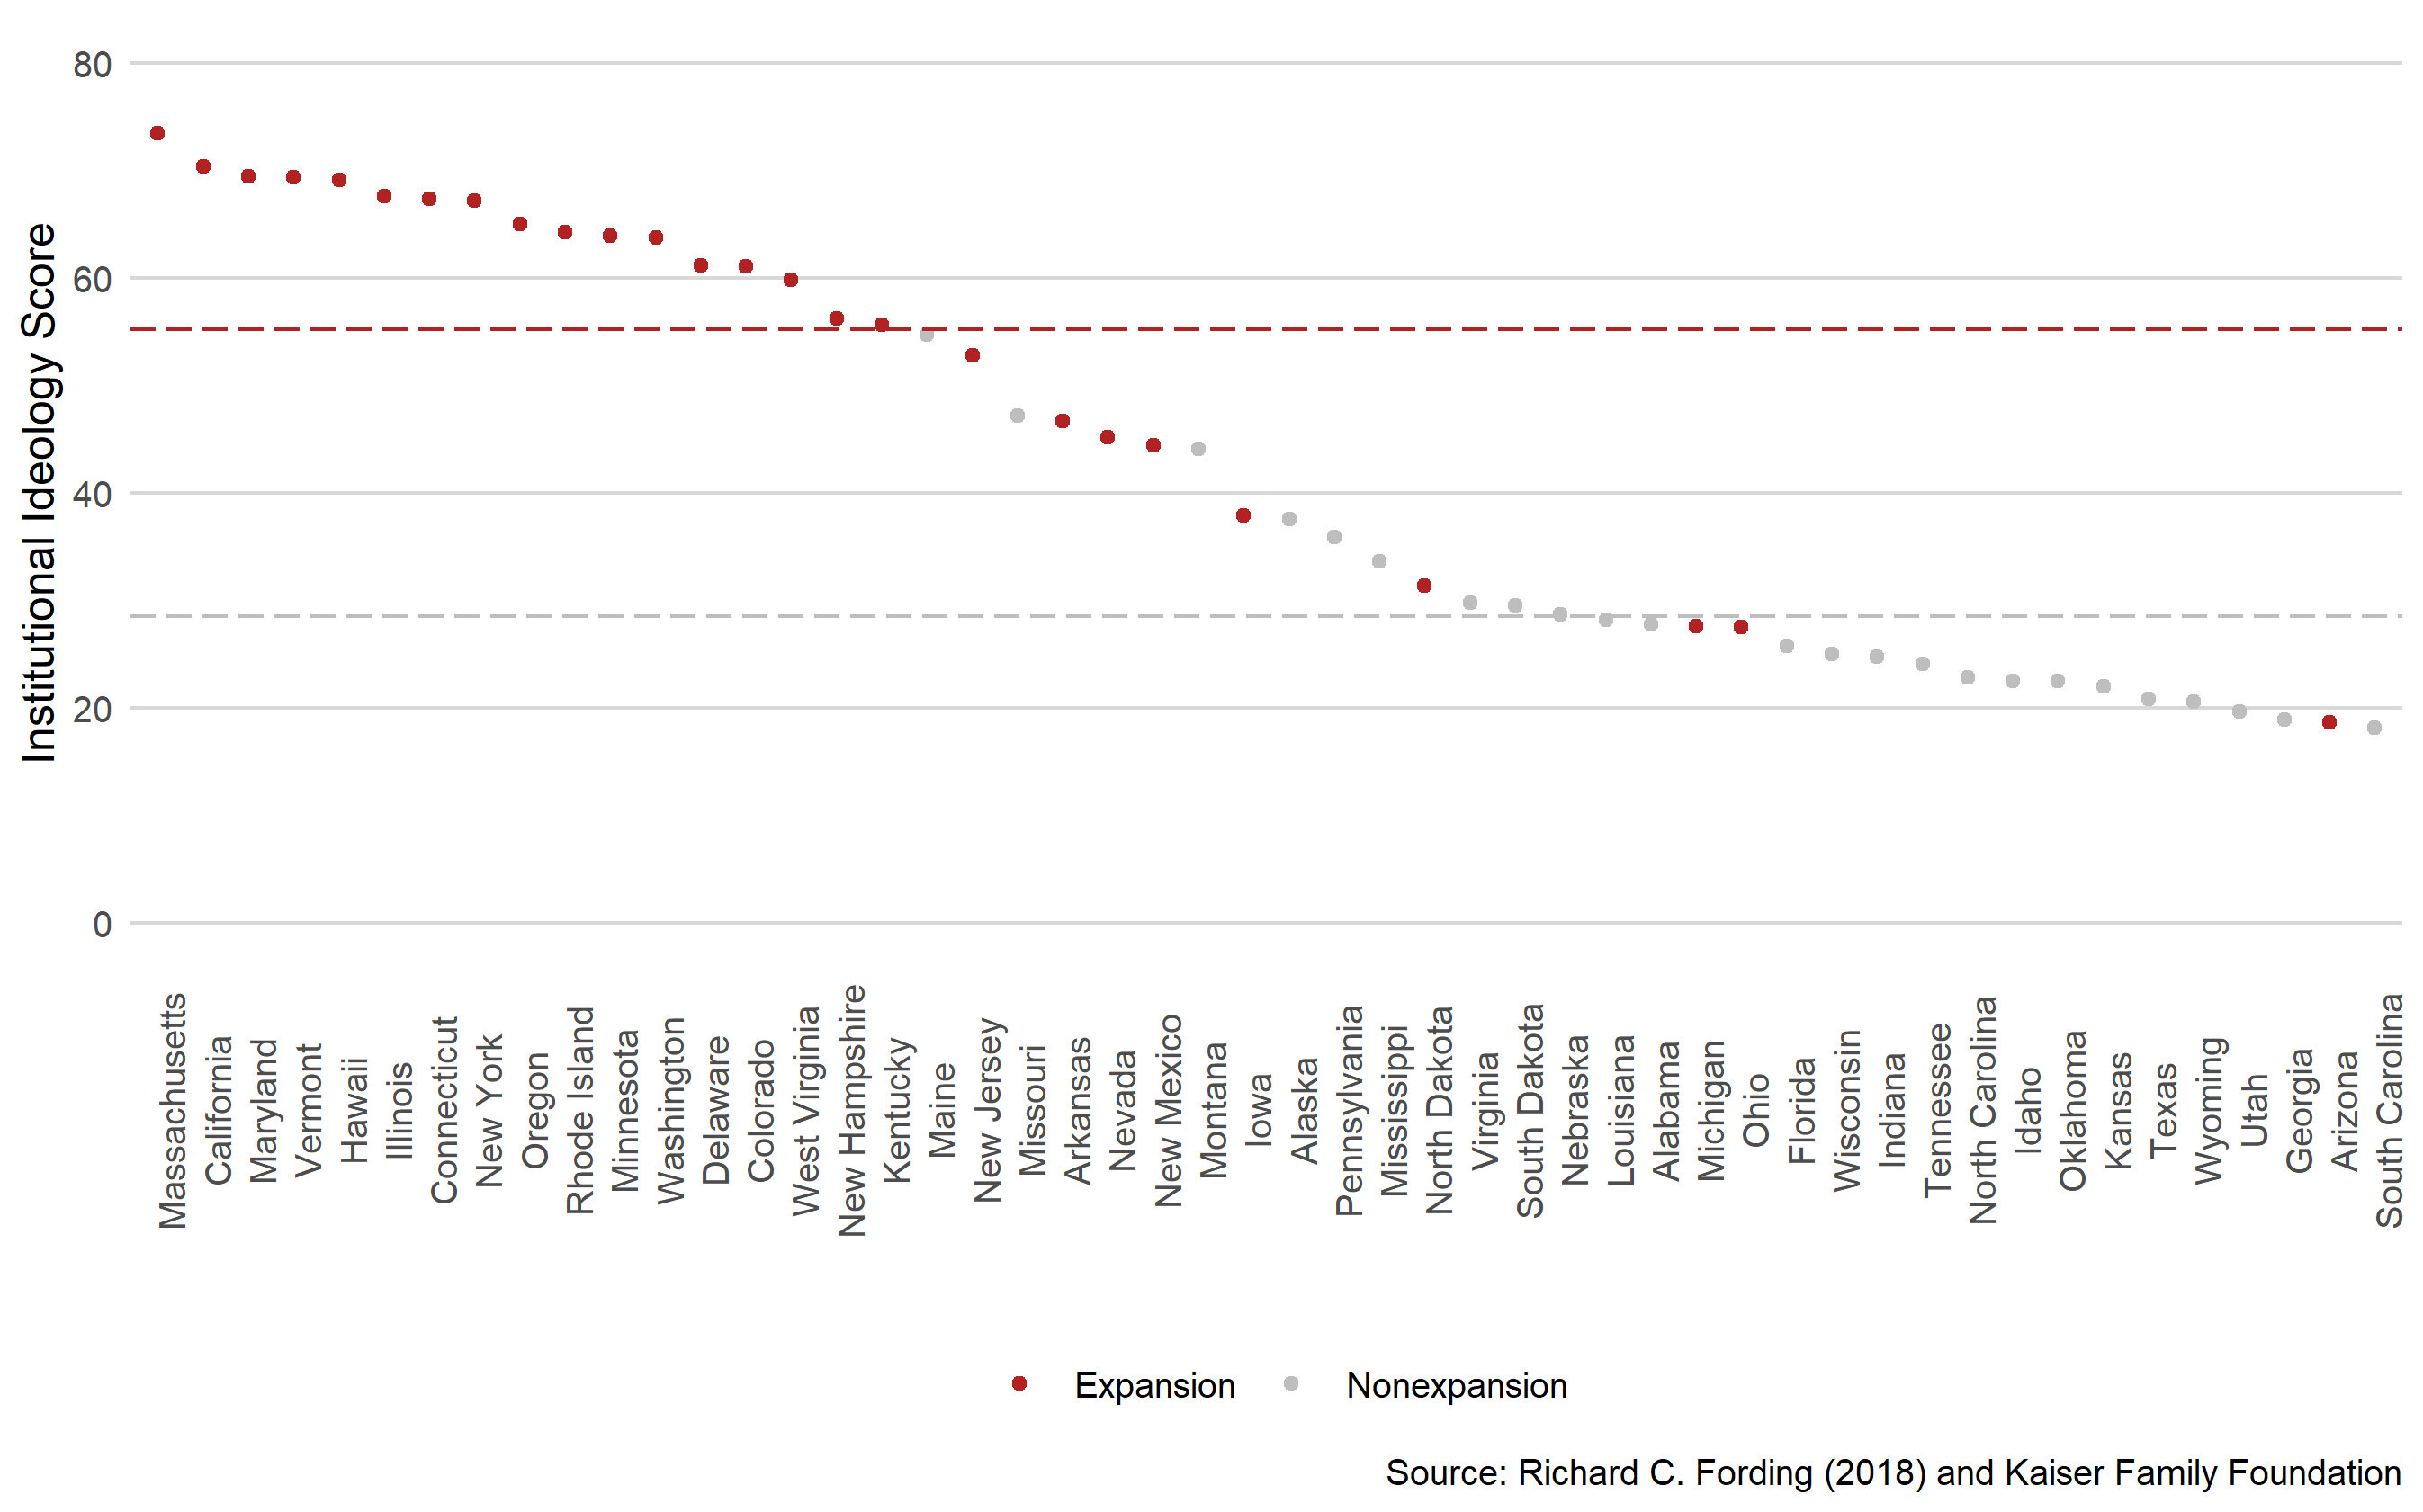
\includegraphics[scale=0.5]{01_Plots/political-expansion-plot.png}
    \end{center}
\end{figure}

Republican governance is not the only source of potential effect heterogeneity. \cite{courtemanche2017early} has previously called attention to how differential uninsurance rates prior to Medicaid expansion is an important effect modifier. Using a difference-in-difference-in-differences strategy, \cite{courtemanche2017early} estimate a statistically significant linear increase in the probability of being insured in 2014 with respect to an area's 2013 uninsurance rate. This finding implies that non-expansion states, which had higher average pre-treatment uninsurance rates, should have a larger magnitude effect. However, we hypothesize that a states' governance may still moderate the treatment effect even after controlling for pre-treatment uninsurance rates, and, at the very least, that it is an important outcome.

We make three methodological contributions to the literature on balancing weights. First, we clarify the required assumptions to use the ``synthetic controls'' framework to estimate the treatment effect on the controls (ETC) using longitudinal data. In brief, while balancing on pre-treatment outcomes alone arguably suffices for some synthetic control applications (see, e.g., \cite{botosaru2017role}), because our goal in this setting is to estimate treatment response, we stress the importance of balancing ``auxillary covariates'' (covariates that are not pre-treatment outcomes) in order to accurately predict the effect of treatment. Moreover, we cannot necessarily leverage pre-treatment data to train our model withouter assumptions. We instead use an implementation of Stable Balancing Weights (\cite{zubizarreta2015stable}) to estimate a set of positive weights to weight the expansion regions to approximately match the covariate distribution of the non-expansion regions, and use our prior knowledge about which covariates likely predict treatment response to choose how to prioritize which covariates to balance.

Our second and third contributions modify the Stable Balancing Weights (SBW) objective function to account for our data structure. In brief, we use data from the American Community Survey (ACS) aggregated to the consistent public use microdata area (CPUMA) level. These regions nest within states, and using these smaller regions allows us to obtain better covariate balance. However, a common assumption in the applied literature is that regions within states contain dependencies that can worsen the efficiency of standard estimation procedures (see, e.g., \cite{cameron2015practitioner}). Using the assumed correlation structure outlined in \cite{kloek1981ols}, our second contribution is to modify the SBW criterion to reduce the variance of our estimator. We call this objective H-SBW, which more evenly disperses the weights across states relative to the SBW solution. Our third contribution is to address the problem of measurement error in our covariates. Because our region-level covariates are estimated from underlying survey data, the sampling variability in the covariate estimates is a form of measurement error that may bias our effect estimates. We therefore extend regression calibration techniques to this setting (see, e.g., \cite{gleser1992importance}). Specifically, we leverage the replicate survey weights provided in the ACS microdata to generate estimates of the true covariate values, which we then use to train our weights. This is the first study we are aware of that attempts to adjust for hierarchical data structure and measurement error in the covariates when using balancing weights.

The remainder of this paper has the following structure. Section 2 provides an overview of the data and defines the study period, covariates, outcome, and treatment. Section 3 discusses our methods, beginning by defining our target estimand, and then outlining our identification, estimation, and inferential procedures. Section 4 presents our results, sensitivity analyses, and investigation of treatment effect heterogeneity. Section 5 contains a discussion of the policy relevance of our findings, and Section 6 contains a brief summary. The Appendices contain additional materials, including proofs, summary statistics, and additional results.
